% do not change this formatting 
\documentclass[10pt, margins = .5in]{article}
\parindent=0pt \parskip=8pt
\textwidth=3in
\hoffset=.3in 
\usepackage{amssymb,amsmath,amsthm,mathrsfs} 
\pagestyle{headings}
\usepackage{amsmath}
\newcommand*{\QEDA}{\hfill\ensuremath{\blacksquare}}%
\usepackage[margin=.5in]{geometry}
\usepackage{xcolor}
\usepackage{amsthm}
\usepackage{url}
\usepackage{shadethm}
\usepackage{mathtools}
\usepackage{systeme}
\usepackage{float}
\usepackage{mathtools}
\setlength\parindent{24pt}
\newcommand\numberthis{\addtocounter{equation}{1}\tag{\theequation}}
\usepackage{caption}
\usepackage{subcaption}
\newtheorem{theorem}{Theorem}
\usepackage{dcolumn}
\newcolumntype{2}{D{.}{}{2.0}}
\usepackage{subfig}
\usepackage{mwe}



\usepackage[utf8]{inputenc}


\begin{document}


\section{Shane's Part}
In two dimensions, one can model the macroscopic behavior of the system by
\begin{equation}
\frac{\partial \rho}{\partial t} = D\Big(\frac{\partial^2 \rho}{\partial^2 x} + \frac{\partial^2 \rho}{\partial^2 y}\Big) + \rho(1-\rho),
\label{eq: Macro2D}
\end{equation}
where $\rho(t,x,y)$ is the density of cancer cell at time $t$ at location $(x,y),$ and $D$ is the diffusion coefficient. One can model the microscopic behavior of the system by 

\begin{equation}
dX_t = \sigma dB_t,
\label{eq: MicroModel2}
\end{equation}
where $\sigma = \sqrt{2D}$, and $B_t$ denotes a standard two-dimensional Brownian motion, with $B(0) = (0,0)$. Thus,

\begin{equation}
\int_0^{\Delta t} \ dX_t = \sigma \int_{0}^{\Delta t} \ dB_t \implies x_{\Delta t} - x_0 = \sigma \textbf{Z}
\end{equation}
where $\textbf{Z} \sim \mathcal{N}_2((0, 0), \Delta t \mathbb{I}_2)$, where $\mathbb{I}_p$is the $p \times p$ identity matrix. We conclude that
\begin{equation}
x_{\Delta t} = x_0 + \sigma \sqrt{\Delta t}\textbf{W},
\label{eq: BrownianEQ}
\end{equation} 
where $\textbf{W} \sim \mathcal{N}_2((0,0), \mathbb{I}_2).$ In Figures \ref{fig:macroPlot} and \ref{fig:microPlot} we plot the level curves of the solution to (\ref{eq: Macro2D}) and (\ref{eq: BrownianEQ}) respectively. We use $N = 10^4, L = M = 5, \Delta x = \Delta y = .2$ at $t = 0,$ where $x \in [-L, L], \ y \in [-M, M]$.
In Figure \ref{fig: WD}, we plot the Wasserstein Distance between the solutions of (\ref{eq: Macro2D}) and (\ref{eq: MicroModel2}) as a function of $t$, where we use $N = 10^3,\ \Delta t = .05, \ t = 20, L = M  = 2, \ \Delta x = \Delta y = .5.$ 

\begin{figure}[H]
\begin{subfigure}{.5\linewidth}
\centering
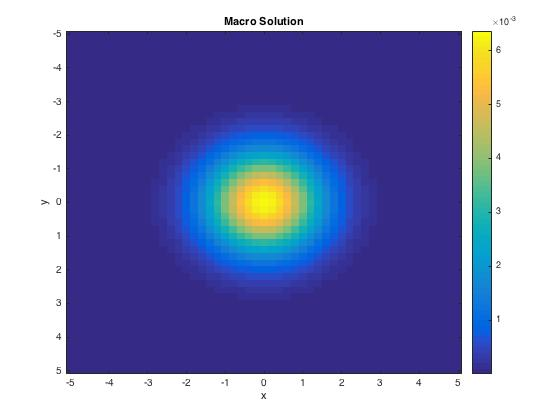
\includegraphics[scale = .40]{MacroPlot.jpg}
\caption{Macro Solution}
\label{fig:macroPlot}
\end{subfigure}%
\begin{subfigure}{.40\linewidth}
\centering
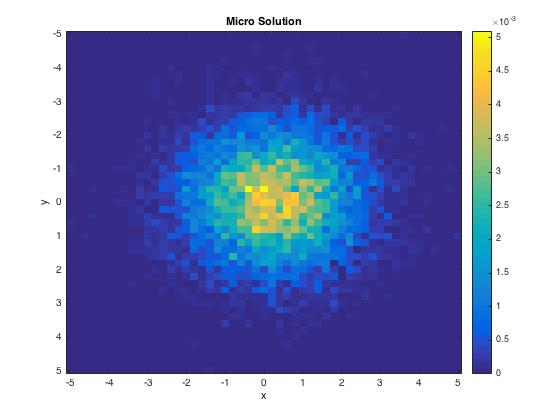
\includegraphics[scale = .40]{MicroPlot.jpg}
\caption{Micro Solution}
\label{fig:microPlot}
\end{subfigure}\\[1ex]
\centering
\begin{subfigure}{.45\linewidth}
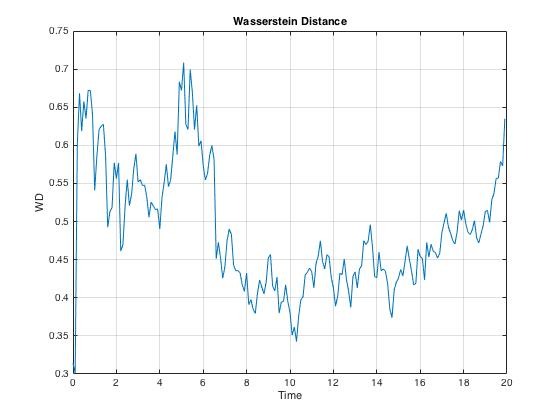
\includegraphics[scale = .45]{WD.jpg}
  \caption{Wasserstein Distance}
\label{fig: WD}
\end{subfigure}
\caption{2D WD Data}
\label{fig:test}
\end{figure}

 
\end{document}
